\documentclass{beamer}
\usetheme{Warsaw}

\usepackage[utf8]{inputenc}
\usepackage{fancybox}
\usepackage{multimedia} 
\usepackage{subfig}
\usepackage{amsmath}
\usepackage{hyperref}
\usepackage[all]{xy}
\begin{document}


\title[Stochastik] % (optional, only for long titles)
{Stochastik für Informatiker
\\
\includegraphics[scale=0.5]{img/craps}
}
\subtitle{}
\author[Dr. Johannes Riesterer] % (optional, for multiple authors)
{Dr.  rer. nat. Johannes Riesterer}

\date[KPT 2004] % (optional)
{}

\subject{Stochastik}


\frame{\titlepage}


\begin{frame}
    \frametitle{Highlight}
\framesubtitle{}
\begin{figure}[htp]
      \centering
    
\includegraphics[width=0.9\textwidth]{img/firework}
\end{figure}
 \end{frame}


\begin{frame}
    \frametitle{Diskrete Wahrscheinlichkeitsverteilung}
\framesubtitle{}

\begin{block}{Beispiel: Hash Kollision}
Beim Hashing werden zufällig $k \leq n$ Daten auf $n$ Speicherplätze  verteilt. Bezeichnen wir mit $A_{k,n}$ die Möglichkeiten der Mehrfachbelegungen von Feldern, so ist das Komplementäre Ereignis
$A^c_{k,n} = Perm^n_k(\Omega, o.W.)$,  wobei $\Omega$ die Menge der Verfügbaren Speicherplätze Darstellt. 
\end{block}


\begin{figure}[htp]
      \centering
    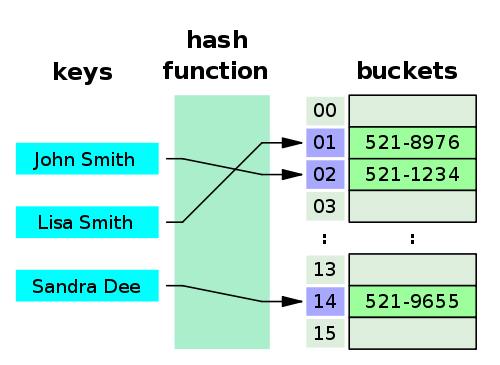
\includegraphics[width=0.5\textwidth]{img/hashtable}

      \caption{Quelle: Wikipedia}
\end{figure}


 \end{frame}


\begin{frame}
    \frametitle{Diskrete Wahrscheinlichkeitsverteilung}
\framesubtitle{}

\begin{block}{Beispiel: Hash Kollision}
\begin{align*}
 P(A^c_{k,n} ) & = \frac{\# Perm^n_k(\Omega, o.W.)}{ \# Perm^n_k(\Omega, m.W.)} = \frac{n_k}{n^k} = \prod_{i=0}^{k-1} (1- \frac{i}{n}) \\
& = \exp (\sum_{i=0}^{k-1} \ln {(1- \frac{i}{n})}) \leq  \exp (\sum_{i=0}^{k-1} (- \frac{i}{n}) \\
 & (ln(1-x) \leq -x \text{ für } x < 1) \\
&= \exp(- \frac{(k-1)k } {2n})
\end{align*}
\end{block}



 \end{frame}

\begin{frame}
    \frametitle{Diskrete Wahrscheinlichkeitsverteilung}
\framesubtitle{}

\begin{block}{Beispiel: Hash Kollision (Geburtstags-Paradoxon)}
Für $n=365$ und $k=23$ ist damit $ P(A_{k,n} ) > \frac{1}{2}$. Die Wahrscheinlichkeit, dass bei einer Gruppe von mehr als $23$ Leuten zwei Leute am gleichen Tag Geburtstag haben, ist also größer als $ \frac{1}{2}$.
\end{block}



 \end{frame}




\begin{frame}
    \frametitle{Axiome von Kolmogorov}
\framesubtitle{}
\begin{block}{$\sigma$-Algebra}
Es sei $\Omega$ eine Menge und $\mathcal{A} \subset  \mathcal{P}(\Omega)$ ein System von Teilmengen. $\mathcal{A}$ heißt $\sigma$-Algebra (Ereignis-Algebra) falls gilt:
\begin{align*}
& (i) \; \Omega \subset \mathcal{A} \\
& (ii) \; A \in \mathcal{A} \Rightarrow A^c \in \mathcal{A} \\
& (iii) \; A_i \in \mathcal{A} \Rightarrow \bigcup_i A_i \in \mathcal{A} 
\end{align*}
$(A^c = \Omega - A)$
\end{block}

\begin{block}{Interpretation}
Die Grundmenge $\Omega$ ist ein Ereignis. Das nicht-Eintreffen eines Ereignisses ist ein Ereignis. Die Vereinigung von Ereignissen ist ein Ereignis.
\end{block}


 \end{frame}


\begin{frame}
    \frametitle{Axiome von Kolmogorov}
\framesubtitle{}
\begin{block}{Axiome von Kolmogorov}
Ein Wahrscheinlichkeitsraum ist ein Tripel $(\Omega, \mathcal{A}, P)$ bestehend aus der Grundmenge $\Omega$, einer $\sigma$-Algebra $\mathcal{A} \subset  \mathcal{P}(\Omega)$ und einer Abbildung
$P : \mathcal{A} \to [0,1]$
\begin{align*}
(i) & \; P(\Omega) = 1 \\
(ii) & \;  P \biggl(  \bigcup_i A_i  \biggr) = \sum_i P(A_i), \text{ mit } A_i \cap A_j = \emptyset \text{ für } i \neq j
\end{align*}
Die Elemente von $\Omega$ werden elementare Ereignisse und die von $\mathcal{A}$ Ereignisse genannt. Mengen mit $P(M) = 0$ werden Nullmengen genannt.
\end{block}


\begin{block}{Interpretation}
Die Grundmenge ist ein sicheres Ereignis. Die Wahrscheinlichkeit von überschneidungsfreien Ereignissen addiert sich.
\end{block}


 \end{frame}





\begin{frame}
    \frametitle{Diskrete Wahrscheinlichkeitsverteilungen}
\framesubtitle{}
\begin{block}{Diskrete Wahrscheinlichkeitsverteilung}
Ein diskreter Wahrscheinlichkeitsraum ist ein Wahrscheinlichkeitsraum $(\Omega, \mathcal{A}, P)$, bei dem die Grundmenge $\Omega$ albzählbar ist.
\end{block}
\begin{block}{Beispiel: Laplace Wahrscheinlichkeit}
$\Omega$ endlich $ \mathcal{A} = \mathcal{P}(\Omega)$,  und $P(A) = \frac{\#A}{\#\Omega}$.
\end{block}

 \end{frame}



\begin{frame}
    \frametitle{Diskrete Wahrscheinlichkeitsverteilungen}
\framesubtitle{}

\begin{block}{Lemma}
Sei $(\Omega, \mathcal{A}, P)$ ein diskreter Wahrscheinlichkeitsraum. Dann ist für $A \subset \mathcal{A}$ 
\begin{align*}
& P(A) = \sum_{\omega \in A} P(\{ \omega \}) \\
& P(A^c) = 1 - P(A) \\
& P(\emptyset) = 0
\end{align*}

\end{block}

 \end{frame}







\begin{frame}
    \frametitle{Diskrete Wahrscheinlichkeitsverteilungen}
\framesubtitle{}

\begin{block}{Herleitung der bedingten  Wahrscheinlichkeit}
\begin{align*}
& \tilde{\Omega} : = B \\
& \tilde{\mathcal{A}} := \{ C \cap B  \; | \;  C \in \mathcal{A} \}  \\
& \tilde{P} = \frac{P }{P(B)}
\end{align*}
\end{block}


\begin{figure}[htp]
      \centering
    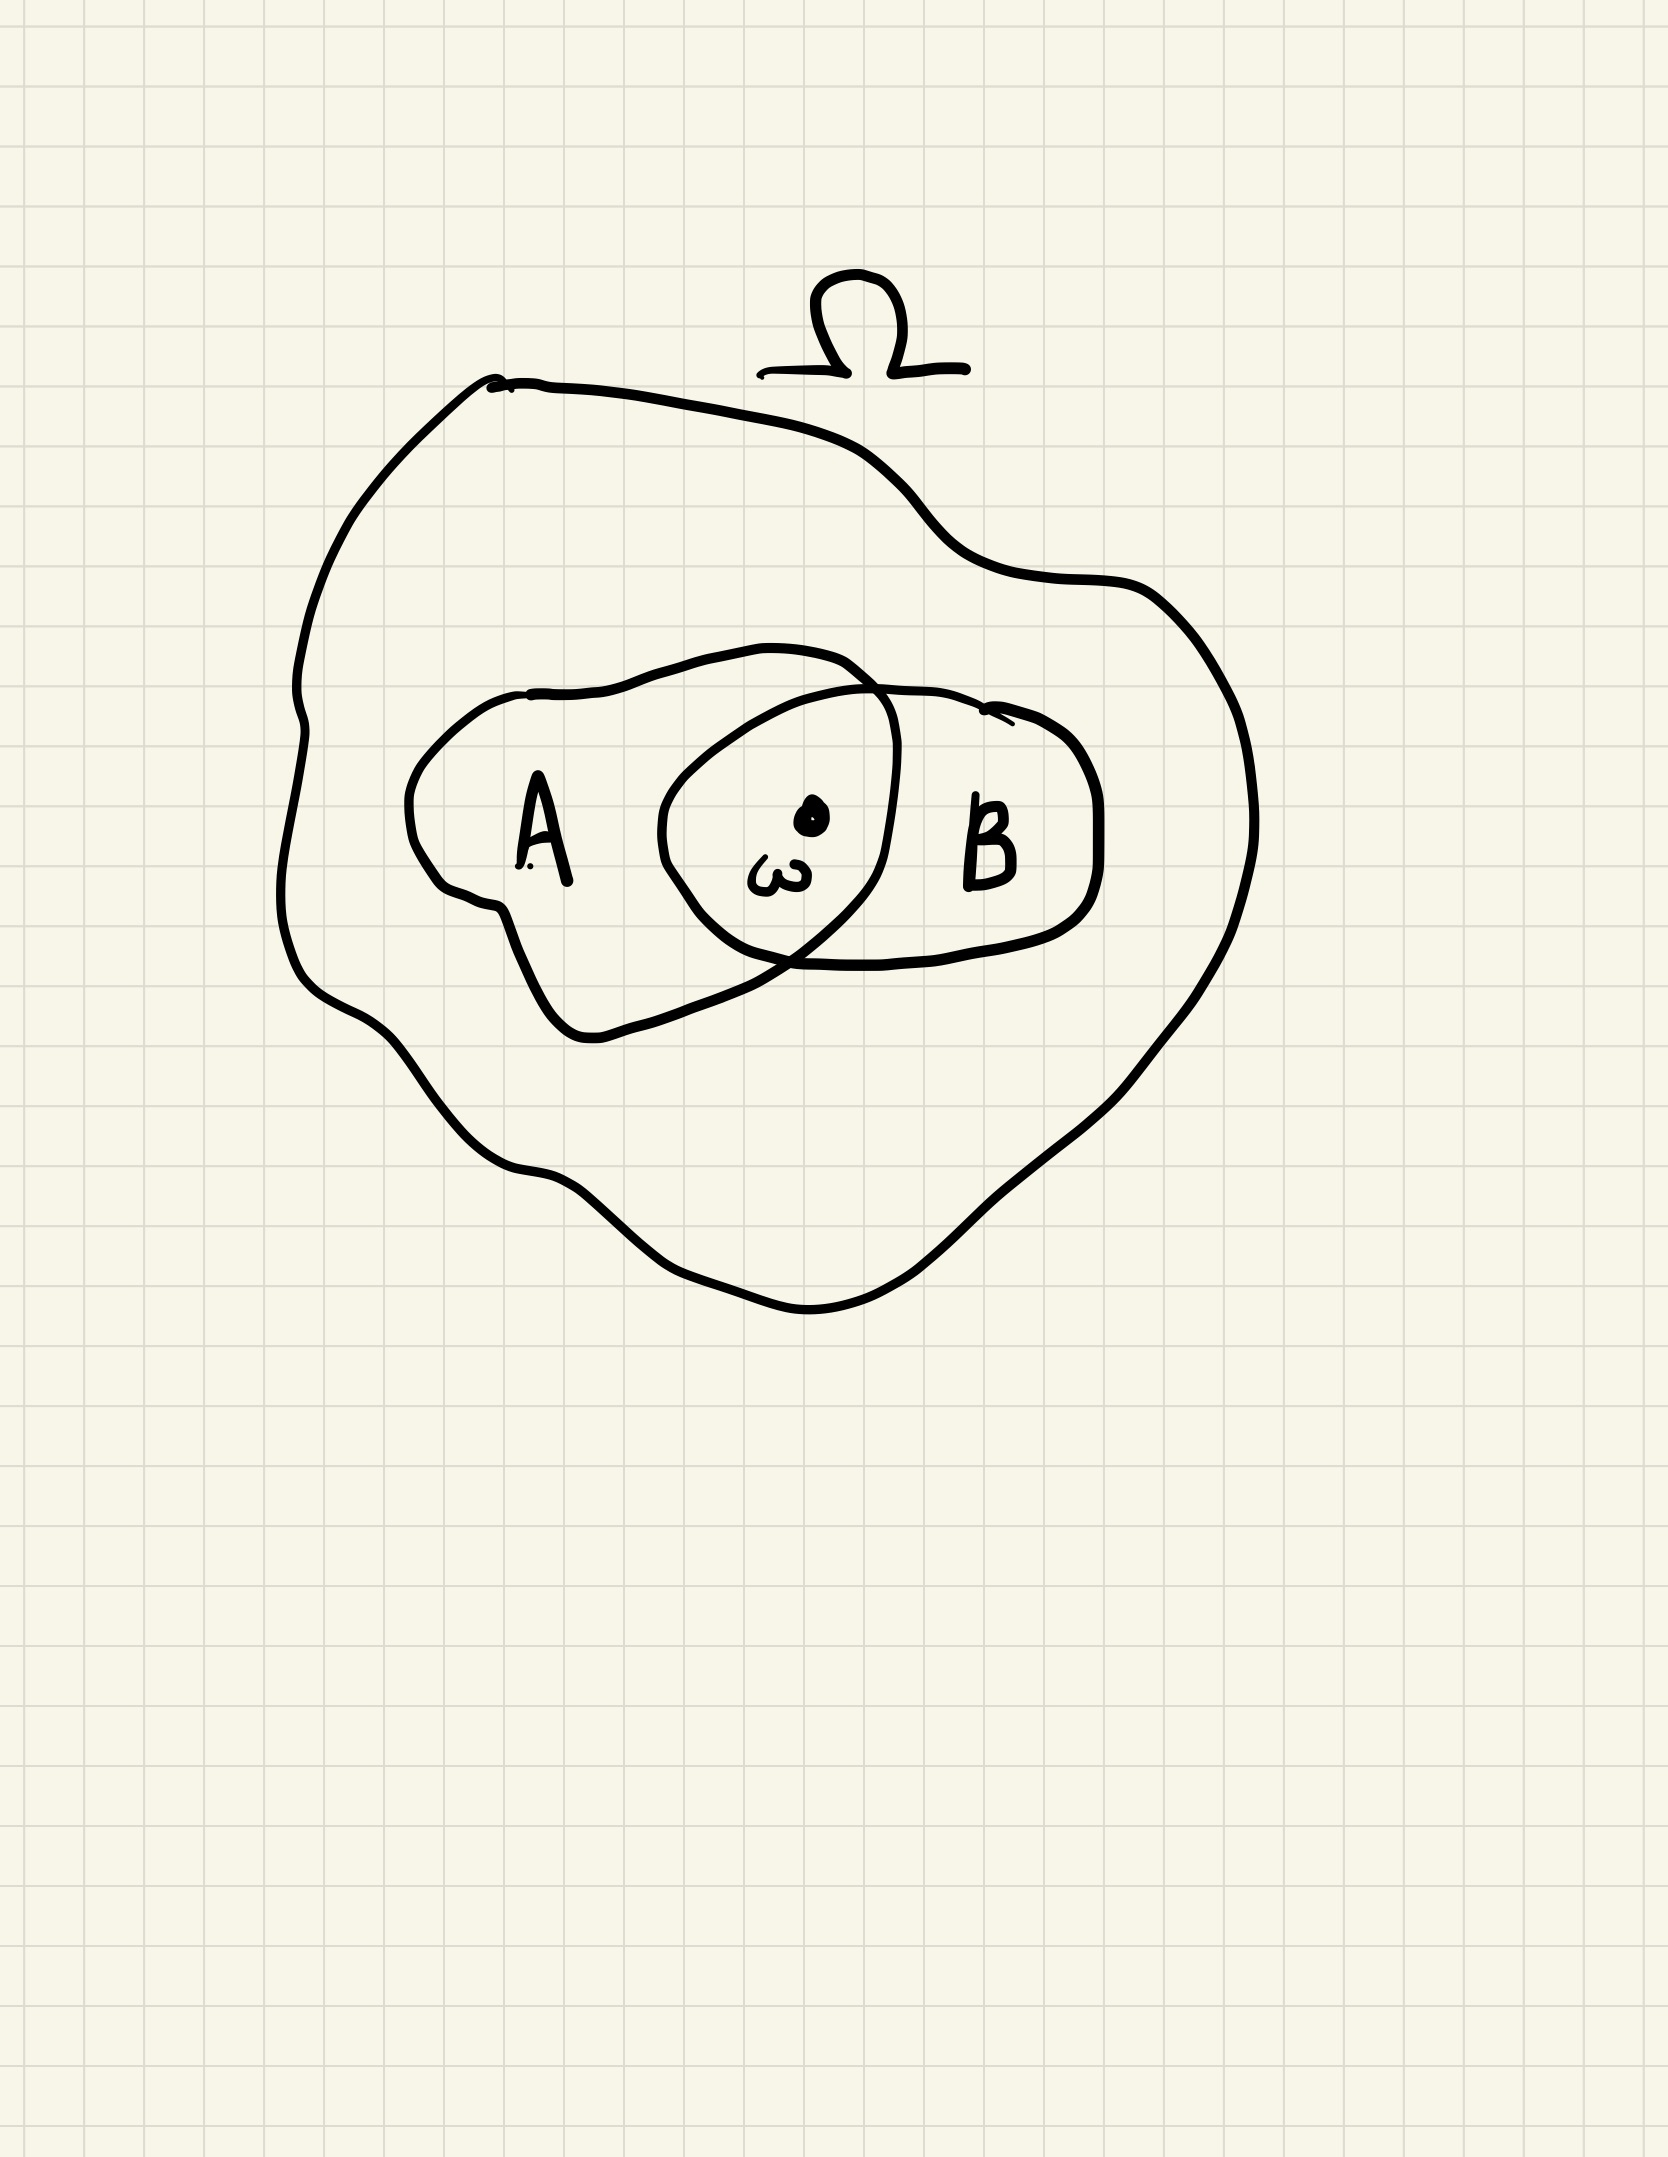
\includegraphics[width=0.3\textwidth]{img/bedingtewkeit}
\end{figure}

 \end{frame}


\begin{frame}
    \frametitle{Diskrete Wahrscheinlichkeitsverteilungen}
\framesubtitle{}

\begin{block}{Bedingte  Wahrscheinlichkeit}
Für $A,B \subset \mathcal{P}(\Omega)$ und $P(B) > 0$ heißt
\begin{align*}
& P(A \; | \;  B) = \frac{P(A \cap B)}{P(B)} \\
\end{align*}
die bedingte Wahrscheinlichkeit (von $A$ unter $B$).
\end{block}


\begin{figure}[htp]
      \centering
    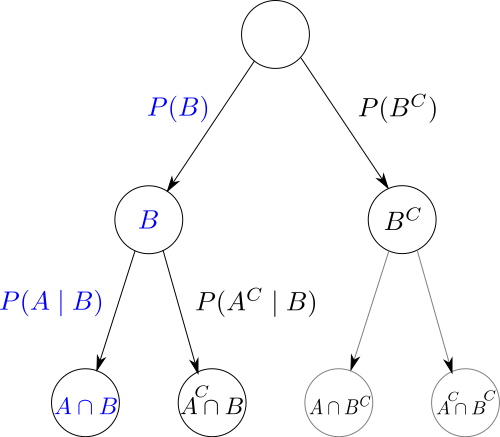
\includegraphics[width=0.3\textwidth]{img/Probability_tree}

      \caption{Quelle: Wikipedia}
\end{figure}

 \end{frame}




\begin{frame}
    \frametitle{Diskrete Wahrscheinlichkeitsverteilung}
\framesubtitle{}

\begin{block}{Satz der totalen Wahrscheinlichkeit}
Für eine Zerlegung  $\Omega = \bigcup_{j=1}^{n} B_j, \text{ mit } B_i \cap B_k = \emptyset \text{ für } i \neq k $
\begin{align*}
& P(A ) = \sum_{j=1}^{n}  P(A \; | \;  B_j) \cdot P(B_j)
\end{align*}
\end{block}

 \end{frame}



\begin{frame}
    \frametitle{Diskrete Wahrscheinlichkeitsverteilung}
\framesubtitle{}

\begin{block}{Satz von Bayes}
Für $A,B \subset \mathcal{P}(\Omega)$ mit  $P(B) > 0$ gilt
\begin{align*}
& P(A \; | \;  B) = \frac{P(B \; | \; A) \cdot P(A)} {P(B)} \\
\end{align*}
\end{block}

\begin{block}{Beweis}
\begin{align*}
& P(A \; | \;  B) =\frac{P(A \cap B)}{P(B)} = \frac{ \frac{P(A \cap B) \cdot P(A)}{P(A)}}{P(B)}  =  \frac{P(B \; | \; A) \cdot P(A)} {P(B)} 
\end{align*}
\end{block}



 \end{frame}



\begin{frame}
    \frametitle{Diskrete Wahrscheinlichkeitsverteilung}
\framesubtitle{}

\begin{block}{Stochastische Unabhängigkeit}
Zwei Ereignisse $A,B$ heißen stochastisch Unabhängig, falls
\begin{align*}
P(A \cap B) = P(A) \cdot P(B)
\end{align*}
gilt.  Gleichbedeutend damit ist  $P(A | B) = P(A)$ und $P(B  | A) = P(B)$.
\end{block}



 \end{frame}


\begin{frame}
    \frametitle{Highlight}
\framesubtitle{}
\begin{figure}[htp]
      \centering
    
\includegraphics[width=0.9\textwidth]{img/firework}
\end{figure}
 \end{frame}


\begin{frame}
    \frametitle{Diskrete Wahrscheinlichkeitsverteilung}
\framesubtitle{}

\begin{block}{Naiver Bayes'scher Spam Filter}
Gegeben ist eine E-Mail $E$.  Wir möchten anhand des Vorkommens bestimmter Wörter $A_1, \ldots A_n$ in der Mail entscheiden, ob es sich um eine erwünschte Mail $H$ oder eine unerwünschte Mail $S$ (Ham or Spam) handelt. 
(Typische Wörter wären zum Beispiel "reichwerden",  "onlinecasino" ...)
\end{block}

\begin{figure}[htp]
      \centering
    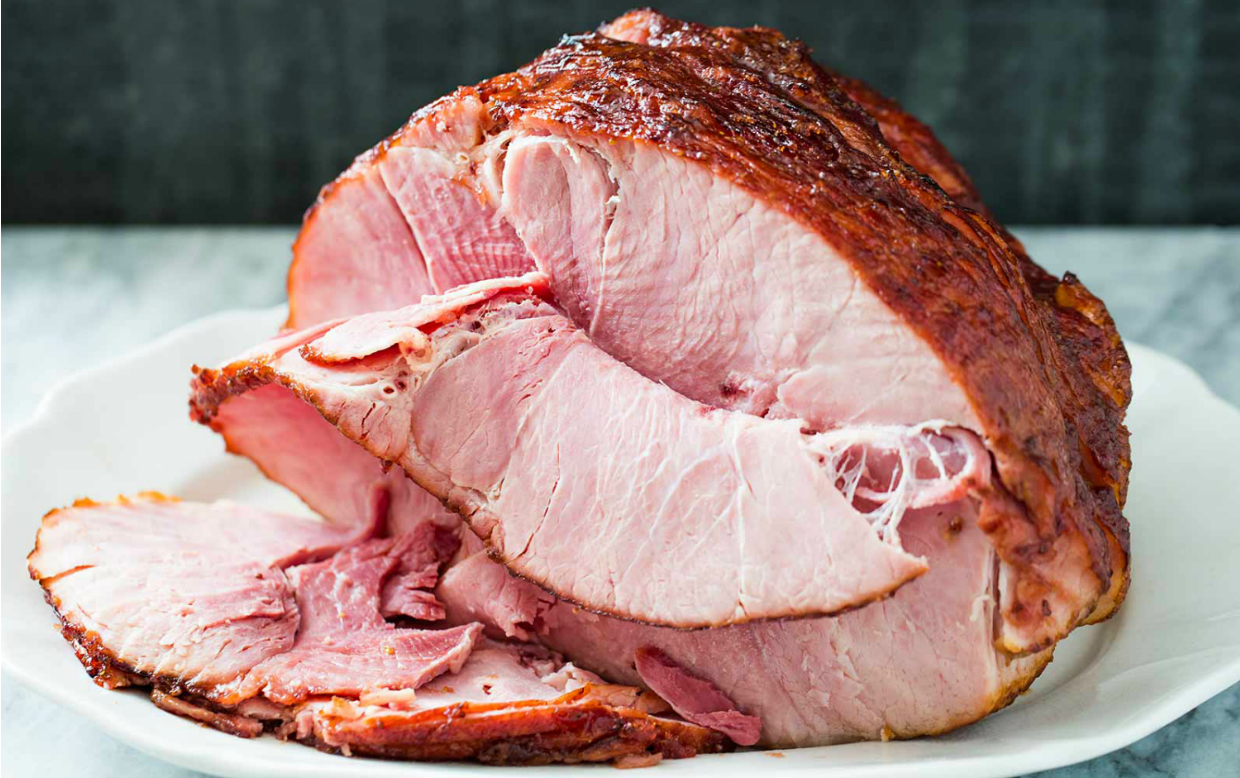
\includegraphics[width=0.4\textwidth]{img/ham}
    
\includegraphics[width=0.4\textwidth]{img/spam}

\end{figure}



 \end{frame}


\begin{frame}
    \frametitle{Diskrete Wahrscheinlichkeitsverteilung}
\framesubtitle{}

\begin{block}{Naiver Bayes'scher Spam Filter}

Aus einer Datenbank kann man das Vorkommen dieser Wörter in Spam und Ham Mails zählen und damit empirisch die Wahrscheinlichkeiten $P(A_i | S)$ und $P(A_i | H) $ des Vorkommens dieser Wörter in Spam und Ham Mails ermitteln.  Wir gehen davon aus, dass es sich bei der Mail  prinzipiell mit  Wahrscheinlichkeit $P(E= S) = P(E= H)= \frac{1}{2}$  um eine erwünschte  Mail $H$ oder eine unerwünschte Mail $S$  handeln kann. 
\end{block}

 \end{frame}



\begin{frame}
    \frametitle{Diskrete Wahrscheinlichkeitsverteilung}
\framesubtitle{}

\begin{block}{Naiver Bayes'scher Spam Filter}
 Wir machen zudem die (naive) Annahme, dass das Vorkommen der Wörter  stochastisch unabhängig ist, also 
\begin{align*}
P(A_1 \cap \cdots \cap A_n | S) = P(A_1 | S) \cdots P(A_n | S) \\
P(A_1 \cap \cdots \cap A_n | H) = P(A_1 | H) \cdots P(A_n | H)
\end{align*}
gilt.
\end{block}

 \end{frame}


\begin{frame}
    \frametitle{Diskrete Wahrscheinlichkeitsverteilung}
\framesubtitle{}

\begin{block}{Naiver Bayes'scher Spam Filter}
Mit der Formel von Bayes und der totalen Wahrscheinlichkeit  können wir somit berechnen
\begin{align*}
& P(E=S |  A_1 \cap \cdots \cap A_n) = \frac{P(A_1 \cap \cdots \cap A_n | S) \cdot P(S)}{P(A_1 \cap \cdots \cap A_n)} \\
&=  \frac{P(A_1 | S) \cdots P(A_n | S) \cdot P(S)}{P(A_1 \cap \cdots \cap A_n | H) + P(A_1 \cap \cdots \cap A_n | S)} \\
&=  \frac{P(A_1 | S) \cdots P(A_n | S) \cdot P(S)}{P(A_1 | H) \cdots P(A_n | H)  + P(A_1 | S) \cdots P(A_n | S) } \\
\end{align*}
Bemerkung: $P(E=H |  A_1 \cap \cdots \cap A_n) = 1- P(E=S |  A_1 \cap \cdots \cap A_n) $
\end{block}



 \end{frame}


\end{document}
